\documentclass[10pt, landscape]{article}
\usepackage[scaled=0.92]{helvet}
\usepackage{calc}
\usepackage{multicol}
\usepackage{ifthen}
\usepackage[a4paper,margin=5mm,landscape]{geometry}
\usepackage{amsmath,amsthm,amsfonts,amssymb}
\usepackage{color,graphicx,overpic}
\usepackage{hyperref}
\usepackage{newtxtext} 
\usepackage{enumitem}
\usepackage{amssymb}
\usepackage[table]{xcolor}
\usepackage{vwcol}
\usepackage{tikz}
\usetikzlibrary{arrows.meta}
\usetikzlibrary{calc}
\usepackage{mathtools}
\usepackage{nicematrix}
\usepackage[T1]{fontenc} %%% <--- NOTE THIS
% for relations
\usepackage{cancel}
\usepackage{ mathrsfs }
\usepackage{listings}
\usepackage{background}
\setlist{nosep}

\usepackage{etoolbox}
\makeatletter
\preto{\@verbatim}{\topsep=0pt \partopsep=0pt }
\makeatother

\backgroundsetup{
scale=1,
color=black,
opacity=0.4,
angle=0,
contents={
  % 
\includegraphics[width=\paperwidth,height=\paperheight]{eldon.png}
  }
}

\pdfinfo{
  /Title (CS2040S.pdf)
  /Creator (TeX)
  /Producer (pdfTeX 1.40.0)
  /Author (Seamus)
  /Subject (Example)
  /Keywords (pdflatex, latex,pdftex,tex)}

\lstset{language=Java,keywordstyle={\bfseries \color{black}}}

% Turn off header and footer
\pagestyle{empty}

\newenvironment{tightcenter}{%
  \setlength\topsep{0pt}
  \setlength\parskip{0pt}
  \begin{center}
}{%
  \end{center}
}

% redefine section commands to use less space
\makeatletter
\renewcommand{\section}{\@startsection{section}{1}{0mm}%
                                {-1ex plus -.5ex minus -.2ex}%
                                {0.5ex plus .2ex}%x
                                {\normalfont\large\bfseries}}
\renewcommand{\section}{\@startsection{section}{2}{0mm}%
                                {-1explus -.5ex minus -.2ex}%
                                {0.5ex plus .2ex}%
                                {\normalfont\normalsize\bfseries}}
\renewcommand{\subsection}{\@startsection{subsection}{3}{0mm}%
                                {-1ex plus -.5ex minus -.2ex}%
                                {1ex plus .2ex}%
                                {\normalfont\small\bfseries}}%
\renewcommand{\familydefault}{\sfdefault}
\renewcommand\rmdefault{\sfdefault}
% makes nested numbering (e.g. 1.1.1, 1.1.2, etc)
\renewcommand{\labelenumii}{\theenumii}
\renewcommand{\theenumii}{\theenumi.\arabic{enumii}.}
\renewcommand\labelitemii{•}
%  for logical not operator
\renewcommand{\lnot}{\mathord{\sim}}
\renewcommand{\bf}[1]{\textbf{#1}}
\newcommand{\abs}[1]{\vert #1 \vert}
\newcommand{\Mod}[1]{\ \mathrm{mod}\ #1}

\makeatother
\definecolor{myblue}{cmyk}{1,.72,0,.38}
\everymath\expandafter{\the\everymath \color{myblue}}
% Define BibTeX command
\def\BibTeX{{\rm B\kern-.05em{\sc i\kern-.025em b}\kern-.08em
    T\kern-.1667em\lower.7ex\hbox{E}\kern-.125emX}}
\let\iff\leftrightarrow
\let\Iff\Leftrightarrow
\let\then\rightarrow
\let\Then\Rightarrow

% Don't print section numbers
\setcounter{secnumdepth}{0}

\setlength{\parindent}{0pt}
\setlength{\parskip}{0pt plus 0.5ex}
%% this changes all items (enumerate and itemize)
\setlength{\leftmargini}{0.5cm}
\setlength{\leftmarginii}{0.5cm}
\setlist[itemize,1]{leftmargin=2mm,labelindent=1mm,labelsep=1mm}
\setlist[itemize,2]{leftmargin=4mm,labelindent=1mm,labelsep=1mm}

%My Environments
\newtheorem{example}[section]{Example}
% -----------------------------------------------------------------------

\begin{document}
\raggedright
\footnotesize
\begin{multicols*}{3}

% multicol parameters
% These lengths are set only within the two main columns
\setlength{\columnseprule}{0.25pt}
\setlength{\premulticols}{1pt}
\setlength{\postmulticols}{1pt}
\setlength{\multicolsep}{1pt}
\setlength{\columnsep}{2pt}

\begin{center}
    \fbox{%
        \parbox{0.8\linewidth}{\centering \textcolor{black}{
            {\Large\textbf{ST2334}}
            \\ \normalsize{AY25/26 Sem 2}}
            \\ {\footnotesize \textcolor{myblue}{by ngmh}} 
        }%
    }
\end{center}

\section{Basic Concepts of Probability}
\textbf{Union}
\begin{itemize}
    \item $A \cup B = \{x:x\in A \lor x \in B\}$
    \item $\bigcup_{i=1}^n A_i=A_1\cup A_2 \cup ... \cup A_n=\{x:x\in A_1 \lor x\in A_2 \lor ... \lor x \in A_n\}$
\end{itemize}

\textbf{Intersection}
\begin{itemize}
    \item $A \cap B = \{x:x\in A \land x \in B\}$
    \item $\bigcap_{i=1}^n A_i=A_1\cap A_2 \cap ... \cap A_n=\{x:x\in A_1 \land x\in A_2 \land ... \land x \in A_n\}$
\end{itemize}

\textbf{Complement} $A'=\{x : x\in S \land x \notin A\}$

\textbf{Mutually Exclusive / Disjoint} $A \cap B = \emptyset$

\textbf{Event Operations}
\begin{itemize}
    \item $A \cap A' = \emptyset$
    \item $A \cap \emptyset = \emptyset$
    \item $A \cup A' = S$
    \item $(A')'=A$
    \item $A \cup (B \cap C) = (A \cup B) \cap (A \cup C)$
    \item $A \cap (B \cup C)=(A\cap B) \cup (A \cap C)$
    \item $A \cup B = A\cup (B \cap A')$
    \item $A = (A \cap B) \cup (A \cap B')$
\end{itemize}

\textbf{De Morgan's Law}
\begin{itemize}
    \item $(A_1 \cup A_2 \cup ... \cup A_n)'=A_1'\cap A_2'\cap ... \cap A_n'$
    \item $(A_1 \cap A_2 \cap ... \cap A_n)'=A_1'\cup A_2'\cup ... \cup A_n'$
\end{itemize}

\textbf{Permutation} Selection and arrangement of $r$ objects out of $n$: $P_r^n=\frac{n!}{(n-r)!}$

\textbf{Combination} Selection of $r$ objects out of $n$ without regards to order: $C_r^n={n \choose r}=\frac{n!}{r!(n-r)!}$, ${n \choose r}={n \choose n-r}$

\textbf{Probability Axioms}
\begin{enumerate}
    \item $0\leq P(A) \leq 1$
    \item $P(S)=1$
    \item $A \cap B = \emptyset \Rightarrow P(A \cup B) = P(A)+P(B)$
\end{enumerate}

\textbf{Basic Properties of Probability}
\begin{enumerate}
    \item $P(\emptyset)=0$
    \item For mutually exclusive events, $P(A_1\cup A_2 \cup... \cup A_n)=P(A_1)+P(A_2)+...+P(A_n)$
    \item $P(A')=1-P(A)$
    \item $P(A)=P(A\cap B)+P(A \cap B')$
    \item $P(A \cup B)=P(A)+P(B)-P(A \cap B)$
    \item If $A \subset B$ then $P(A)\leq P(B)$
\end{enumerate}

\textbf{Conditional Probability} The probability of $B$ given $A$ occurring is $P(B|A)=\frac{P(A\cap B)}{P(A)}$

\textbf{Multiplication Rule} $P(A\cap B)=P(A)P(B|A)=P(B)P(A|B)$ given $P(A) \neq 0$ or $P(B) \neq 0$

\textbf{Inverse Probability Formula} $P(A|B)=\frac{P(A)P(B|A)}{P(B)}$

\textbf{Independence} $P(A\cap B)=P(A)P(B)$, denoted $A \perp B$

\textbf{Some Properties of Independence}
\begin{itemize}
    \item If $P(A)>0, P(B) > 0, A \perp B$, then $A$ and $B$ are not mutually exclusive
    \item If $P(A)>0, P(B)>0,$ and they are mutually exclusive, then $A \not\perp B$
    \item $S$ and $\emptyset$ are independent of any other event
    \item If $A \perp B$, then $A \perp B', A' \perp B, A' \perp B'$
\end{itemize}

\textbf{Partition} For mutually exclusive events with $\bigcup^n_{i=1}A_i=S$, $A_1,A_2,...,A_n$ is a partition of $S$

\textbf{Law of Total Probability} For a partition of $S$, $P(B)=\sum_{i=1}^nP(B \cap A_i)=\sum_{i=1}^nP(A_i)P(B|A_i)$

\textbf{Baye's Theorem} For a partition of $S$, $P(A_k|B)=\frac{P(A_k)P(B|A_k)}{\sum_{i=1}^nP(A_i)P(B|A_k)}$

\section{Random Variables}
\textbf{Probability Mass Function for Discrete Random Variables}
\[
f(x)=\begin{cases}
    P(X=x) & x \in R_X \\
    0 & x \notin R_X \\
    \end{cases}
\]
\begin{enumerate}
    \item $f(x_i) \geq 0$ for all $x_i \in R_X$
    \item $f(x)=0$ for all $x \notin R_X$
    \item $\sum_{i=1}^\infty f(x_i)=1$
\end{enumerate}

\textbf{Probability Density Function for Continuous Random Variables}
\begin{enumerate}
    \item $f(x) \geq 0$ for all $x \in R_X$, $f(x)=0$ for all $x \notin R_X$
    \item $\int_{R_X}f(x)dx=1$
    \item For $a \leq b$, $P(a \leq X \leq b)=\int_a^b f(x) dx$
\end{enumerate}
It suffices to check conditions 1 and 2

\textbf{Cumulative Distribution Function} $F(x)=P(X \leq x)$
\begin{itemize}
    \item Discrete RV: $F(x)=\sum_{t\in R_X, t \leq x}P(x=t)$, $P(a \leq X \leq b)=F(b)-F(a-)$
    \item Continuous RV: $F(x)=\int_{-\infty}^x f(t)dt$, $f(x)=\frac{dF(x)}{dx}$, $P(a \leq X \leq b) = F(b)-F(a)$
\end{itemize}

\textbf{Expectation / Mean}
\begin{itemize}
    \item Discrete RV:  $\mu_X=E(X)=\sum_{x_i\in R_X} x_if(x_i)$
    \item Continuous RV: $\mu_X=E(X)=\int_{-\infty}^{\infty}xf(x)dx=\int_{x\in R_X}xf(x)dx$
\end{itemize}

\textbf{Properties of Expectation}
\begin{enumerate}
    \item $E(aX+b)=aE(X)+b$
    \item $E(X+Y)=E(X)+E(Y)$
    \item For arbitrary $g(.)$
    \begin{itemize}
        \item Discrete RV: $E[g(X)]=\sum_{x\in R_X}g(x)f(x)$
        \item Continuous RV: $E[g(X)]=\int_{R_X}g(x)f(x)dx$
    \end{itemize}
\end{enumerate}

\textbf{Variance and Properties} $\sigma_X^2=V(X)=E(X-\mu_X)^2$
\begin{itemize}
    \item Discrete RV: $V(X)=\sum_{x\in R_X}(x-\mu_X)^2f(x)$
    \item Continuous RV: $V(X)=\int_{-\infty}^\infty (x-\mu_X)^2f(x)dx$
    \item $V(X)\geq 0$ for any $X$, with equality holding iff $P(X=E(X))=1$
    \item $V(aX+b)=a^2V(X)$
    \item Alternative Formula: $V(X)=E(X^2)-[E(X)]^2$
\end{itemize}

\textbf{Standard Deviation} $\sigma_X=\sqrt{V(X)}$, $\sigma_X \geq 0$

\section{Joint Distributions}
\textbf{Discrete Joint Probability Function} $f_{X,Y}(x, y)=P(X=x, Y=y)$, $(x,y)\in R_{x, y}$
\begin{enumerate}
    \item $f_{X,Y}(x,y)\geq0$, $(x, y) \in R_{X,Y}$
    \item $f_{X,Y}(x,y)=0$, $(x, y) \notin R_{X,Y}$
    \item $\sum_{i=1}^\infty \sum_{j=1}^\infty f_{X,Y}(x_i,y_j)=\sum_{i=1}^\infty \sum_{j=1}^\infty P(X=x_i, Y=y_j)=1$ or $\sum\sum_{(x,y)\in R_{X,Y}}f(x,y)=1$
    \item $P((X, Y) \in A)=\sum\sum_{(x,y)\in A}f(x,y)$
\end{enumerate}

\textbf{Continuous Joint Probability Function} $P((X, Y)\in D)=\int\int_{(x, y) \in D}f_{X, Y}(x, y)dy dx$, or $P(a \leq X \leq b, c \leq Y \leq d)=\int_a^b\int_c^df_{X, Y}(x, y)dy dx$
\begin{enumerate}
    \item $f_{X, Y}(x, y) \geq 0$, $(x, y) \in R_{X, Y}$
    \item $f_{X, Y}(x, y) = 0$, $(x, y) \notin R_{X, Y}$
    \item $\int_{-\infty}^\infty\int_{-\infty}^\infty f_{X, Y}(x, y) dx dy = 1$ or $\int\int_{(x, y) \in R_{X, Y}}f_{X, Y}(x, y)dx dy=1$
\end{enumerate}

\textbf{Marginal Probability Distribution} Projection of 2D function onto 1D function
\begin{itemize}
    \item Y Discrete: $f_X(x)=\sum_yf{X, Y}(x, y)$
    \item Y Continuous: $f_X(x)=\int_{-\infty}^\infty f_{X, Y}(x, y)dy$
\end{itemize}

\textbf{Conditional Distribution} Distribution of $Y$ given that $X$ is observed, $f_{Y|X}(y|x)=\frac{f_{X, Y}(x, y)}{f_X(x)}$
\begin{enumerate}
    \item Defined for $f_X(x)>0$
    \item If $f_X(x)>0$, then $f_{X, Y}(x, y)=f_X(x)f_{Y|X}(y|x)$
    \item $P(Y \leq y | X=x)=\int_{-\infty}^y f_{Y|X}(y|x)dy$
    \item $E(Y|X=x)=\int_{-\infty}^\infty y f_{Y|X}(y|x)dy$
\end{enumerate}

\textbf{Independent Random Variables} $X_1, X_2, ..., X_n$ are independent iff $f_{X_1, X_2, ..., X_n}(x_1, x_2, ..., x_n)=f_{X_1}(x_1)f_{X_2}(x_2)...f_{X_n}(x_n)$. $R_{X, Y}$ must be a product space of $R_X \times R_Y$ by satisfying all possibilities.

\textbf{Properties of Independent Random Variables}
\begin{enumerate}
    \item $P(X \in A; Y \in B)=P(X\in A)P(Y \in B)$, for any real $x, y$, $P(X \leq x; Y \leq y)=P(X \leq x)P(Y \leq y)$
    \item For arbitrary $g_1(.)$ and $g_2(.)$, $g_1(X)$ and $g_2(Y)$ are independent
    \item If $f_X(x) > 0$, then $f_{Y|X}(y|x)=f_Y(y)$
\end{enumerate}

\textbf{Checking Independence}
\begin{enumerate}
    \item $R_{X, Y}$ where the probability function is positive must be a product space
    \item For $(x, y) \in R_{X, Y}$, $f_{X, Y}(x, y)=C \times g_1(x) \times g_2(y)$, i.e. it can be factorised into terms independent of other variables
\end{enumerate}

\textbf{Marginal Distribution under Independence} Given $g_1(x)$ and $g_2(y)$,
\begin{itemize}
    \item X Discrete: Probability mass function is $f_X(x)=\frac{g_1(x)}{\sum_{t \in R_X}g_1(t)}$
    \item X Continuous: Probability density function is $f_X(x)=\frac{g_1(x)}{\int_{t \in R_X} g_1(t)dt}$
\end{itemize}

\textbf{Expectation}
\begin{itemize}
    \item Discrete: $E(g(X, Y))=\sum_x\sum_y g(x, y)f_{X, Y}(x, y)$
    \item Continuous: $E(g(X, Y))=\int_{-\infty}^\infty\int_{-\infty}^\infty g(x, y) f_{X, Y}(x, y)dydx$
\end{itemize}

\textbf{Covariance} $cov(X, Y)=E[(X-E(X))(Y-E(Y))]$ using $g(X, Y)=(X-E(X))(Y-E(Y))$
\begin{itemize}
    \item Discrete: $cov(X, Y)=\sum_x\sum_y(x-\mu_X)(y-\mu_Y)f_{X, Y}(x, y)$
    \item Continuous: $cov(X, Y)=\int_{-\infty}^\infty\int_{-\infty}^\infty(x-\mu_X)(y-\mu_Y)f_{X, Y}(x, y)dxdy$
\end{itemize}

\textbf{Properties of Covariance}
\begin{enumerate}
    \item $cov(X, Y)=E(XY)-E(X)E(Y)$
    \item If $X$ and $Y$ are independent, $cov(X, Y)=0$, and $E(XY)=E(X)E(Y)$
    \item $cov(aX+b, cY+d)=ac \cdot cov(X, Y)$ using $cov(X+b, Y)=cov(X, Y)$ and $cov(aX, Y)=acov(X, Y)$
    \item $V(aX+bY)=a^2V(X)+b^2V(Y)+2ab\cdot cov(X, Y)$ using $V(X+Y)=V(X)+V(Y)+2cov(X, Y)$
\end{enumerate}

\textbf{Properties of Variance and Covariance}
\begin{enumerate}
    \item For independent $X$ and $Y$, $V(X \pm Y)=V(X)+V(Y)$
    \item $V(X_1+X_2+...+X_n)=V(X_1)+V(X_2)+...+V(X_n)+2 \sum_{j > i}cov(X_i, X_j)$
    \item For independent $X_1, X_2, ... , X_n$, $V(X_1\pm X_2 \pm ... \pm X_n)=V(X_1)+V(X_2)+...+V(X_n)$
\end{enumerate}

\section{Special Probability Distributions}
\subsection{Discrete Distributions}
\textbf{Discrete Uniform Distribution} The random variable assumes discrete values with equal probability
\begin{itemize}
    \item pmf: $1/k$ if there are $k$ values it can take on
    \item $\mu_X=E(X)=\frac{1}{k}\sum_{i=1}^kx_i$
    \item $\sigma_X^2=V(X)=E(X^2)-[E(X)]^2=\frac{1}{k}\sum_{i=1}^k x_i^2-\mu_X^2$
\end{itemize}

\textbf{Bernoulli Trial} Random experiment with only two possible outcomes

\textbf{Bernoulli Random Variable $X \sim Bernoulli(p)$} Success of a Bernoulli trial
\begin{itemize}
    \item pmf: $p, x= 1$; $1-p=q, x = 0$
    \item $f_X(x)=p^x(1-p)^{1-x}$, $x=0, 1$
    \item $\mu_X=E(X)=p$
    \item $\sigma_X^2=V(X)=p(1-p)=pq$
\end{itemize}

\textbf{Bernoulli Process} Sequence of repeatedly performed independent and identical Bernoulli trials

\textbf{Binomial Random Variable $X\sim Bin(n, p)$} Counts number of successes in $n$ trials of a Bernoulli Process
\begin{itemize}
    \item $P(X=x)={n\choose x}p^x(1-p)^{n-x}$, $0 \leq x \leq n$
    \item $E(X)=np$
    \item $V(X)=np(1-p)$
\end{itemize}

\textbf{Negative Binomial Distribution $X\sim NB(k, p)$} Let $X$ be the number of independent and identically distributed Bernoulli trials needed until the $k$th success occurs. Then $X$ follows a Negative Binomial Distribution.
\begin{itemize}
    \item pmf: $f_X(x)=P(X=x)={x-1 \choose k-1}p^k(1-p)^{x-k}$, $x\geq k$
    \item Derived from $k-1$ success in first $x-1$ trials and success on $x$th trial
    \item $E(X)=\frac{k}{p}$
    \item $V(X)=\frac{(1-p)k}{p^2}$
\end{itemize}

\textbf{Geometric Distribution $X\sim Geom(p)$} Let $X$ be the number of independent and identically distributed Bernoulli trials needed until the first success occurs. Then $X$ follows a geometric distribution.
\begin{itemize}
    \item pmf: $f_X(x)=P(X=x)=(1-p)^{x-1}p$
    \item $E(X)=\frac{1}{p}$
    \item $V(X)=\frac{1-p}{p^2}$
\end{itemize}

\textbf{Poisson Random Variable $X \sim Poisson(\lambda)$} $X$ denotes the number of events occurring in a fixed period of time or fixed region, $\lambda$ is the expectation.
\begin{itemize}
    \item pmf: $f_X(k)=P(X=k)=\frac{e^{-\lambda}\lambda^k}{k!}$, $k \geq 0$, $k$ is the number of occurrences
    \item $E(X)=\lambda$
    \item $V(X)=\lambda$
    \item If $X \sim Poisson(\lambda_1), Y \sim Poisson(\lambda_2), X+Y \sim Poisson(\lambda_1+\lambda_2), (X | X+Y=n) \sim Bin(n, p=\frac{\lambda_1}{\lambda_1+\lambda_2})$
\end{itemize}

\textbf{Poisson Process} A continuous time process where we count number of occurrences within some interval of time. The defining properties of a Poisson process with rate parameter $\alpha$ are
\begin{itemize}
    \item the expected number of occurrences in an interval of length $T$ is $\alpha T$
    \item there are no simultaneous occurrences
    \item the number of occurrences in disjoint time intervals are independent
\end{itemize}
The number of occurrences in any interval $T$ of a Poisson process follows a $Poisson(\alpha T)$ distribution

\textbf{Poisson Approximation to Binomial} Let $X \sim Bin(n, p)$. Suppose $n \rightarrow \infty$ and $p \rightarrow 0$ such that $\lambda=np$ remains constant. Then $X \sim Poisson(np)$. The approximation is good when $n \geq 20, p \leq 0.05$, or $n \geq 100, np \leq 10$

\subsection{Continuous Distributions}
\textbf{Continuous Uniform Distribution $X\sim U(a, b)$}
\begin{itemize}
    \item pdf: $\frac{1}{b-a}$, $a \leq x \leq b$
    \item $E(X)=\frac{a+b}{2}$
    \item $V(X)=\frac{(b-a)^2}{12}$
    \item cdf: $\frac{x-a}{b-a}$, $a \leq x \leq b$
\end{itemize}

\textbf{Exponential Distribution $X \sim Exp(\lambda)$}
\begin{itemize}
    \item pdf: $f_X(x)=\lambda e^{-\lambda x}$, $x \geq 0, \lambda > 0$
    \item $E(X)=\frac{1}{\lambda}$
    \item $V(X)=\frac{1}{\lambda^2}$
    \item cdf: $F_X(x)=1-e^{-\lambda x}$, $x \geq 0$
    \item $P(X>x)=e^{-\lambda x}, x > 0$
    \item Alternatively, $\mu=1/\lambda$, $f_X(x)=\frac{1}{\mu}e^{-x/\mu}$, $E(X)=\mu$, $V(X)=\mu^2$, $F_X(x)=1-e^{-x/\mu}$
    \item $P(X>s+t|X>s)=P(X>t)$, i.e. the distribution is "memoryless"
\end{itemize}

\textbf{Normal Distribution $X\sim N(\mu, \sigma^2)$}
\begin{itemize}
    \item pdf: $f_X(x)=\frac{1}{\sqrt{2\pi}\sigma}e^{-(x-\mu)^2/(2\sigma^2)}$
    \item $E(X)=\mu$
    \item $V(X)=\sigma^2$
    \item The total area under the curve is 1
    \item Two curves with the same $\sigma^2$ have identical shapes, but different centers if they have different $\mu$
    \item As $\sigma$ increases, the curve flattens, and vice versa
    \item $X+Y \sim (\mu_1+\mu_2, \sigma_1^2 + \sigma^2_2)$
\end{itemize}

\textbf{Standardised Normal Distribution} Given $X\sim N(\mu, \sigma^2)$, let $Z=\frac{X-\mu}{\sigma}$.
\begin{itemize}
    \item  $Z \sim N(0, 1)$, pdf: $f_Z(z)=\frac{1}{\sqrt{2\pi}}exp(-\frac{z^2}{2})$
    \item For $P(x_1<X<x_2)$, transform it to $z_1, z_2$. Then $P(x_1<X<x_2)=P(z_1<Z<z_2)$
    \item $\phi(.)$ and $\Phi(.)$ denote pdf and cdf of the standard normal
    \item Then $P(x_1<X<x_2)=\Phi(z_2)-\Phi(z_1)$
    \item $P(Z \geq 0) = P(Z\leq 0)=\Phi(0)=0.5$
    \item $\Phi(z)=P(Z \leq z)=P(Z \geq -z)=1-\Phi(-z)$
    \item $Z\sim N(0, 1) \Rightarrow -Z \sim N(0, 1)$
    \item $Z \sim N(0, 1) \Rightarrow \sigma Z + \mu \sim N(\mu, \sigma^2)$
\end{itemize}

\textbf{Quantile} The $\alpha$th (upper) quartile, $0 \leq \alpha \leq 1$, of $X$, is the number $x_\alpha$ such that $P(X \geq x_\alpha)=\alpha$. For $Z$, the $\alpha$th (upper) quartile or $100\alpha$ percentage point is $P(Z \geq z_\alpha)=\alpha$.

\textbf{Normal Approximation to Binomial} Let $X\sim Bin(n, p)$, $E(X)=np$, $V(X)=npq$. As $n \rightarrow\infty$, $Z=\frac{X-E(X)}{\sqrt{V(X)}}=\frac{X-np}{\sqrt{np(1-p)}}$ is approximately $\sim N(0, 1)$, when $np>5$ and $nq>5$

\textbf{Continuity Correction} Accounts for discreteness when approximating to normal, basically when equal, shift outwards, when not equal, shift inwards
\begin{itemize}
    \item $P(X=k)\approx P(k-0.5<X<k+0.5)$
    \item $P(a\leq X \leq b)\approx P(a-0.5<X<b+0.5)$
    \item $P(a < X < b)\approx P(a+0.5<X<b-0.5)$
\end{itemize}

\section{Bell Curve}
\begin{center}
    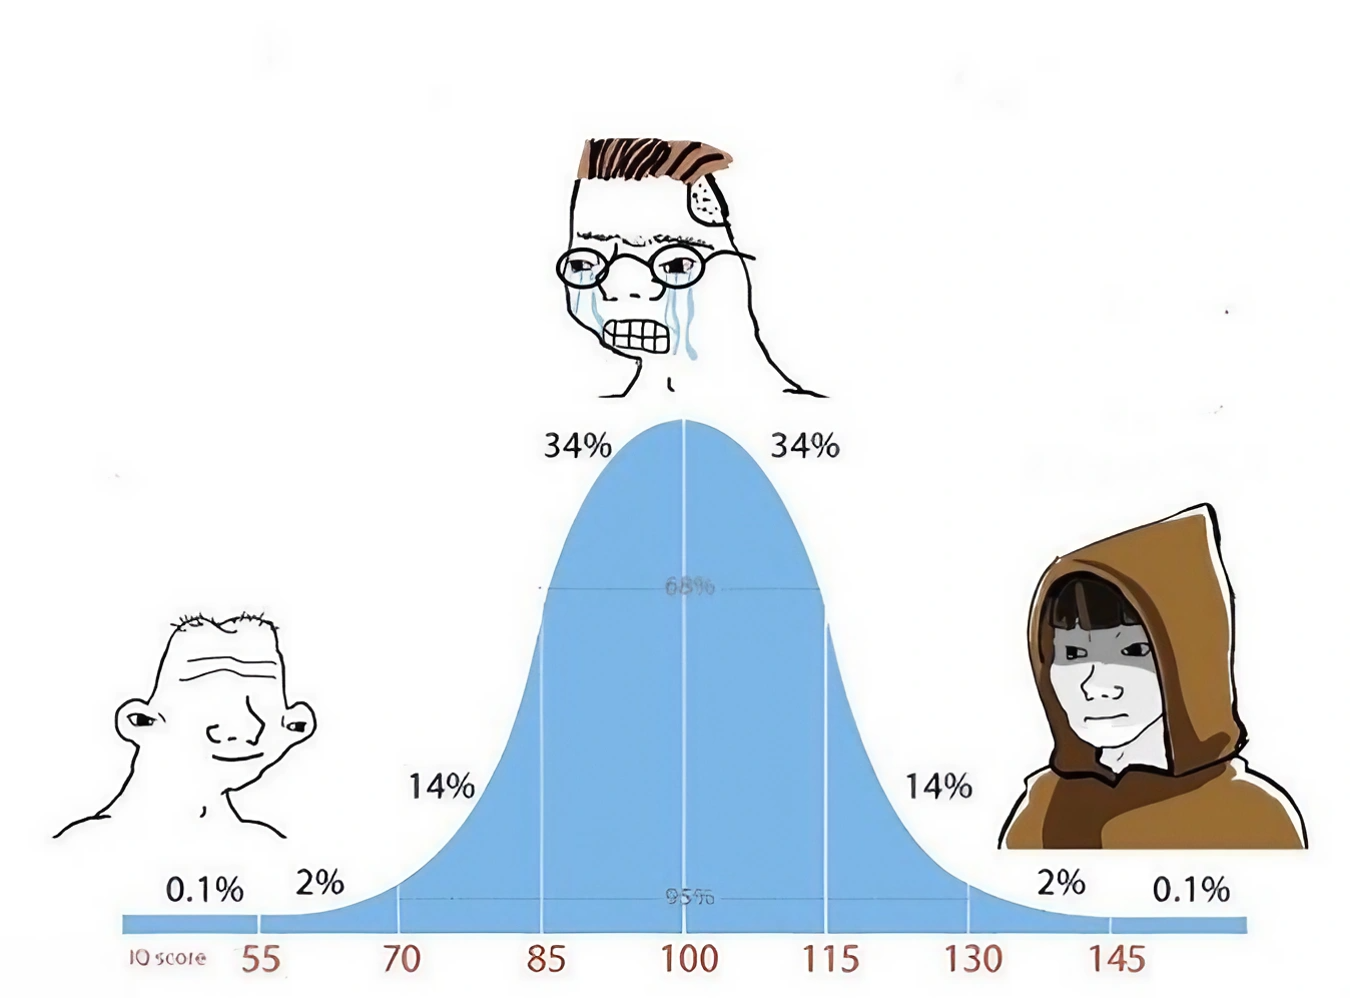
\includegraphics[width=1\linewidth]{curve.png}
\end{center}

\section{Monty Hall Problem}
\begin{center}
    
\includegraphics[width=1\linewidth]{monty.png}
\end{center}

\section{Skewed Curve}
\begin{center}
    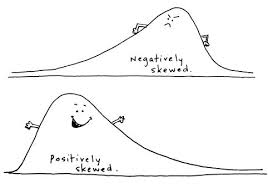
\includegraphics[width=1\linewidth]{happy.png}
\end{center}

\end{multicols*}

\end{document}